\part{Constituer un corpus de petites annonces}



\chapter{Récupérer les journaux d'annonces}

Une fois choisis les journaux d’annonces qui constitueront le corpus\footnote{La constitution détaillée du corpus, comprenant notamment le nombre de numéros récupérés par année, est disponible en annexe.}, j’ai employé des méthodes de \textit{web scraping} pour récupérer leurs versions numérisées sur les bibliothèques numériques de chaque ville : Gallica pour les \textit{Affiches} de Paris, Numelyo pour Lyon, Séléné pour Bordeaux. 

\section{Les \textit{Affiches} de Paris}

Le journal d’annonces de Paris au XVIIIè siècle,\textit{ Annonces, affiches et avis divers} (parfois\textit{ Affiches, annonces et avis divers}), est disponible sur Gallica de 1752 à 1814. Pour récupérer les numéros disponibles, j’ai choisi d’utiliser le \textit{wrapper} Pyllica, qui est spécialement conçu pour la récupération de périodiques via l’API IIIF. En effet, là où d’autres librairies Python (PyGallica, Gallipy) fonctionnent avec l’identifiant d’un document unique, Pyllica permet d’extraire un ensemble de numéros de journaux en précisant le nombre de documents à extraire et la fréquence d’extraction. Pyllica fonctionne sur la base de deux scripts : un premier qui définit une fonction d’extraction jpgpress ; un second qui appelle la fonction, dont l’utilisateur doit alors préciser les paramètres : url gallica du périodique à extraire, titre du fichier à créer, date de début d’extraction, nombre de numéros à extraire, fréquence d’extraction (tous les x jours), nombre de pages par numéro. Par exemple, l'exportation de trente et un numéros quotidiens, de la première à la trentième page, à partir du 1er janvier 1800, se fera avec les paramètres suivants:

\bigskip

\fbox{%
	\begin{minipage}{0.8\textwidth}
		from pyllicalabsjpgpress import *
		
		jpgpress(url="https://gallica.bnf.fr/ark:/12148/cb32683112b/date",
		title="journal", 
		year=1800, month=1, day=1, 
		item=31, rate=1, 
		firstpage=1, lastpage=30)
	\end{minipage}
}




\bigskip

Avant de parvenir à récupérer les images, il m’a fallu amender le premier script, qui répondait aux anciennes normes de Gallica (début d’adresses web en http au lieu de https). En sortie, on obtient ainsi un ensemble d’images jpg, intitulées au format « titre\_année\_mois\_jour\_page ».

Le nombre de numéros disponibles par an varie : pour la majorité des années, surtout de 1752 à 1780, l’intégralité des parutions hebdomadaires (environ 52 numéros par an) ou bihebdomadaires (environ 100 numéros par an) est numérisée. Dans ce cas-là, le choix a été fait de récupérer un numéro par semaine, afin de limiter le temps de récupération, et par commodité par rapport à la méthode de récupération choisie. En effet, Pyllica permet de récupérer des numéros de périodique tous les x jours de publication : on peut choisir de récupérer tous les numéros d’un quotidien en choisissant un pas d’un jour, ou tous les numéros d’un hebdomadaire en choisissant un pas de sept jours, mais les parutions bi-hebdomadaires nécessitent de faire tourner le script deux fois. 

Parfois, l’intégralité ou presque des journaux est disponible, mais les numéros ont été numérisés en une, deux, cinq ou dix fois, sans distinction des numéros par date de parution ; le document numérisé est par exemple mis à la date du 1er janvier de l’année, et fait alors plusieurs centaines de pages d’un coup. C’est le cas des années 1781, 1782, 1789, 1790, 1793, 1794. Dans ce cas, j’ai choisi de ne pas récupérer les journaux, jugeant que le travail de séparation et de datation de chaque numéro serait trop important.

Enfin, pour les numéros du début du XIXè siècle, j’ai fait le choix de récupérer l’ensemble des numéros disponibles, et plus seulement 52 par an, afin de pallier à l’absence de numérisation de nombreuses années de cette période (seules 1804, 1807, 1808 et 1814 sont disponibles) et de rééquilibrer le corpus par rapport aux années 1750-1780. Malheureusement, des restrictions de serveur liées à une refonte de l’API de Gallica m’ont empêchée de récupérer les numéros de 1808 et 1814. 



\section{Les \textit{Affiches} de Lyon}

Les \textit{Affiches} de Lyon, quant à elles, ont été numérisées de 1750 à 1804, avec d’importantes lacunes, notamment entre 1772 et 1795. Elles ont été récupérées à partir de la bibliothèque numérique de la ville de Lyon, Numelyo. Contrairement à Paris et Bordeaux, les numéros étaient cette fois rassemblés par année ou par ensemble de deux ou trois années. Après les avoir téléchargés, il a donc fallu disséquer les documents et leur assigner une date de parution précise. La tâche a été simplifiée par le fait que les numéros font en grande majorité quatre pages, publiés à intervalles réguliers, ce qui a permis d’automatiser une partie du processus ; mais certaines exceptions (suppléments ou compléments publiés en dehors des jours habituels, jours de fêtes qui empêchent la publication…) ont nécessité une vérification à la main. 


\section{Les \textit{Affiches} de Bordeaux}

La récupération des \textit{Annonces, affiches et avis divers pour la ville de Bordeaux} a été la moins automatique, et la moins complète. En effet, la bibliothèque numérique de la ville (Séléné) ne dispose pas d’API, et il n’a pas non plus été possible de récupérer les images disponibles à l’aide d’un script Python et de la librairie \textit{request}, les images étant mises en ligne à l’aide d’un lecteur pdf intégré.
Pour les vingt-trois années disponibles en ligne, de 1758 à 1784, j’ai donc fait le choix de télécharger à la main un numéro par mois. Les \textit{Affiches} de Bordeaux seront donc employées surtout à des fins de comparaison avec Paris et Lyon ; leur mode de récupération les rendent évidemment très minoritaires dans le corpus.

\bigskip

Une fois extraites les images disponibles pour les trois villes, j’ai cherché à unifier et à préparer au mieux mon corpus pour l’océrisation. J’ai tout d’abord utilisé un script Python pour uniformiser les noms de fichiers au format « Annonces\_ville\_année\_mois\_jour\_page ». Pour Bordeaux, j’ai converti les images de pdf à jpg avant de rassembler les images dans des dossiers par ville, puis par année, puis par mois.



\chapter{Océriser les journaux d'annonces}

\section{Un premier essai infructueux avec Tesseract}

Face à la qualité médiocre de l’OCR interne de Gallica, et surtout face à l’absence d’océrisation disponible pour Lyon et Bordeaux, j’ai tout d’abord envisagé d’utiliser le logiciel de reconnaissances optiques de caractères Tesseract. Néanmoins, après l’avoir testé en ligne de commande sur quelques numéros, j’ai pu observer que l’algorithme de Tesseract produisait beaucoup d’erreurs, notamment en tentant d’océriser tout ce qui n’était pas du texte au sein du journal (enjolivures en haut et bas de page, ornements autour des titres, caractères spéciaux à visée décorative, …). De plus, l’algorithme, peu adapté aux documents historiques, performait assez mal lorsque la numérisation était imparfaite, que les caractères étaient légèrement effacés par le temps, ou dès qu’il y avait des tâches sur les pages. Pour la petite dizaine de pages que j’ai testée avec Tesseract, j’ai ainsi obtenu des taux d’erreurs caractères (\textit{Character Error Rate}, ou CER) compris entre 5 et 10 \%, et des taux d’erreurs mots (\textit{Word Error Rate}, ou WER) compris entre 10 et 20 \%. Ces scores ne sont pas complètement mauvais mais ne représentent pas non plus une performance d’océrisation assez bonne pour les usages que je souhaitais faire des petites annonces.


\section{Le choix de Pero-OCR}

Après avoir envisagé un temps d’entraîner Tesseract sur mon corpus (une perspective abandonnée par manque de temps), j’ai ensuite pu tester, grâce à une suggestion de Marie Puren, l’algorithme de Pero-OCR. Pero est un moteur OCR conçu dans le cadre d’un projet entre l’université de technologie de Brno et la bibliothèque morave (République tchèque) visant à développer des outils pour l’exploitation et l’océrisation de documents historiques imprimés. Il a tout particulièrement été entraîné sur des journaux et des documents tchèques de basse qualité des XVIIIè et XIXè siècles\footnote{Ces informations sont disponibles sur le site du projet PERO: https://pero.fit.vutbr.cz/, ainsi que sur le Github du projet: https://github.com/DCGM/pero-ocr}, mais produit de bonnes performances pour la plupart des langues en alphabet latin, y compris le français\footcites{birkholzEvaluatingMultilingualCapabilities2021}. Par ailleurs, il dispose d’une interface en ligne, qui m’a permis de tester l’algorithme avant de l’implémenter grâce à la librairie Python associée. J’ai constaté à la suite de ces premiers tests que l’océrisation avec Pero était très bonne ; en calculant les scores d’erreurs mots et caractère, j’ai observé que ceux-ci se situaient en moyenne aux alentours de 1 \%, souvent pour des erreurs assez négligeables, d’accents ou de signes de ponctuation. Ayant jugé que ces résultats étaient déjà suffisamment bons sans avoir besoin de corriger et de relancer un entraînement de l'algorithme, je n’ai pas utilisé cette fonctionnalité de l’interface en ligne. Je suis donc passée directement à l’élaboration d’un script Python pour l’océrisation des journaux d’annonces.


Ce script prend en entrée les fichiers jpg ou tif des journaux numérisés, et me fournit en sortie des fichiers XML comprenant à la fois les informations de segmentation des pages et d’océrisation du texte. Le processus d’océrisation via la librairie Python repose sur la fonction « process\_page » , et sur un fichier de configuration (dans mon cas, le fichier « config\_file.ini » fourni intialement avec la librairie ; en cas d’entraînement de Pero sur l’interface web, il est possible de générer d’autres fichiers .ini adaptés). Par ailleurs, le script utilise la librairie de traitement d’image OpenCV pour lire les documents d’entrée page par page. Pour obtenir un fichier XML en sortie, j’ai utilisé la fonction « to\_pagexml ». 

\bigskip

\begin{lstlisting}[language=Python,caption=Code Pero-OCR]

import os
import configparser
import cv2
from pero_ocr.document_ocr.layout import PageLayout
from pero_ocr.document_ocr.page_parser import PageParser

path="./Annonces"

os.chdir(path)
for subdir,dirs,files in os.walk(path, topdown=True):
for file in files:
if file.endswith(".jpg") or file.endswith(".tif"):
path_file=os.path.join(path, subdir)
os.chdir(path_file)

# configuration
config_path = "./pero-ocr-modele/config.ini"
config = configparser.ConfigParser()
config.read(config_path)
page_parser = PageParser(config, config_path=os.path.dirname(config_path))
input_image_path = os.path.join(path_file, file)

# lecture de l'image
image = cv2.imread(input_image_path, 1)
page_layout = PageLayout(id=input_image_path,page_size=(image.shape[0], image.shape[1]))

# OCR
page_layout = page_parser.process_page(image, page_layout)

# nouveau dossier pour stocker l'OCR
path_resultats="./OCR_Annonces"
os.chdir(path_resultats)
nom_dossier_resultats="OCR_"+os.path.splitext(os.path.basename(path_file))[0]
if not os.path.exists(nom_dossier_resultats):
os.mkdir(nom_dossier_resultats)
new_path_resultats=os.path.join(path_resultats, nom_dossier_resultats)
os.chdir(new_path_resultats)
nom_fichier='OCR_'+os.path.splitext(os.path.basename(file))[0]+'.xml'

# enregistrement du fichier XML
page_layout.to_pagexml(nom_fichier)
			
\end{lstlisting}

\bigskip
		

\begin{table}[!htbp]
	\centering
	\begin{tabularx}{\textwidth}{|X|X|X|}
		\toprule
		\textbf{\textit{Gold standard} : texte transcrit à la main}        & \textbf{Tesseract (WER=13.1\%; CER=6.6\%)}                              & \textbf{Pero-OCR (WER=1.7\%; CER=0.6\%})  \\
		\midrule
		(935) donner des nouvelles à M. Simon, marché St.-Jean, no 3, recevra la récompense promise. DEMANDES. On desireroit trouver à louer aux environs de Paris, soit à Passy, Auteuil, Chaillot, Meudon, etc., une petite MAISON sise en bon air, ou un Appartement complet, pour trois mois de la belle saison. S'ad. par écrit ou verbalement, au portier du bureau de ce Journal. Demander la lettre D. On desireroit louer ou acheter une petite MAISON de campa- gne à Fontenay-aux-Roses, Meudon, ou à pareille distance de Paris, dans le prix de 10 à 15,000 fr. On voudroit qu'il y eût petit bâtiment et grand jardin. S'ad. par écrit à M. Levol, chef de bureau à l'hôtel de la Monnoie. Une personne âgée de 26 ans, sachant faire une cuisine bour- geoise, coudre, blanchir et parfaitement soigner les enfans, desireroit trouver une PLACE chez une personne de l'un ou l'autre sexe, soit pour Paris ou la campagne. S'adr. rue Coquillère, no. 52, au second, la porte à gauche. Une personne âgée de 32 ans, sachant faire une cuisine bourgeoise, coudre, blanchir et faire tout ce qui concerne le ménage, desireroit se PLACER dans une maison honnête (...). & . 7. “ | oo ( 935 ) donnerà des nouvelles à M. Simon , marche St.-Jean, no. 3, recevra la récompense promise, oo DEMANDES. Où desireroit trouver à louer aux environs de Paris , soit à Passÿ, Aateuil, Chaillot, Meudon , etc., une petite Maxon êise eu bon air, où uu Appartement complet, pour treis mois de la belle saison. S’ad. par écrit ou verbalement , au portier du bureau de ce Journal. Demander la lettre D. | Oa desireroit louer ov acheter une petite Muisow de campa- gne à Foutenay-aux-Roses, Meudon , ou à pareille distance de Paris, dans le-px de 10 à 16,000 fr. On voudroit qu’il y eùt petit bâtiment et grand jardin. S’ad. par écrit à M. Levol, chef de bureau à l’hôtel de la Monnoie. L ” Une personne âgée de 26 ans, sachant faire une cuisine boure geoise, coudre , blanchir et parfailement soigner les enfans, desiréroit trouver une PLace chez une personne de l’un ou l’autre sese, Soit pour Paris ou la campagne. S’adr. rue Coquilière, no. 52, au second, la porte à gauche. lÜae personne âgée de 32 ans , sachant faire une cuisine bourgeoise, coudre, blanchir et faire tout ce qui concerne le ménage, desireroit se PLacEr dans une maison honnête (...) & ( 935 donnera des nouvelles à M. Simon, marché St.-Jean, no. 3, recevra la récompense promise. DEMANDES On desireroit trouver à louer aux environs de Paris, soit à Passy, Auteuil, Chaillot, Meudon, etc., une petite MAISON sise en bon air, ou un Appartement complet, pour trois mois de la belle saison. S'ad. par écrit ou verbalement, au portier du bureau de ce Journal. Demander la lettre D. On desireroit louer ou acheter une petite MAISON de campa- gne à Fontenay-aux-Roses, Meudon, ou à pareille distance de Paris, dans le prix de 10 à 15,000 fr. On voudroit qu'il y eût petit bâtiment et grand jardin. S'ad. par écrit à M. Levol, chef de bureau à l'hôtel de la Monnoie. Une personne âgée de 26 ans, sachant faire une cuisine bour- geoise, coudre, blanchir et parfaitement soigner les enfans, desireroit trouver une PLACE chez une personne de l'un ou l'autre sexe, soit pour Paris ou la campagne. S'adr. rue Coquilière , no. 32, au second, la porte à gauche. Une personne âgée de 32 ans, sachant faire une cuisine bourgeoise, coudre, blanchir et faire tout ce qui concerne le ménage, desireroit se PLACER dans une maison honnête (...) \\ 
		\bottomrule
	\end{tabularx}
	\caption{Comparaison des résultats OCR des deux algorithmes testés (ici sur la page 11 du numéro du 1er mars 1807 des \textit{Affiches de Paris})}
\end{table}%

Le gain en précision de l’OCR avec le passage à Pero s’est fait aux dépends de l’efficacité de l’algorithme : celui-ci est beaucoup plus lent que Tesseract, et prend entre quatre et cinq minutes pour traiter un numéro de journal de quatre pages. Pour les quelques 2700 numéros qui composent mon corpus, cela représente plus de 200 heures de traitement ; il m’a donc fallu décomposer les journaux en plusieurs groupes et faire tourner mon script graduellement. À terme, j’ai donc obtenu un fichier XML par page numérisée. À l’aide de la librairie lxml, j’ai ensuite extrait les résultats de l’océrisation des fichiers XML vers des fichiers txt, que j’ai concaténés afin d’obtenir un seul fichier texte par numéro de journal. 

Une fois l'océrisation complète, et après observation d'une partie des résultats, j'ai employé des expressions régulières afin de corriger certaines erreurs récurrentes: présence d'espaces superflus,"sachant" parfois océrisé en "sachaut", points de ponctuation parfois océrisés en étoiles (*),  s longs corrigés en s dans un souci d'uniformité du corpus.


\chapter{Segmenter, sélectionner, corriger et pré-traiter les annonces}

\section{Des journaux aux annonces: le processus de segmentation}

Plusieurs options ont été envisagées pour segmenter les journaux et parvenir à extraire les annonces individuellement. Une première, inspirée du projet SoDUCo (\textit{Social Dynamics in Urban Context}, ISC-PIF) et de son traitement des annuaires du XIXè siècle, consistait en l'entraînement d'un modèle d'apprentissage profond sur la base de pages annotées à la main. Néanmoins, par souci de temps, une approche plus simple, à base d'expressions régulières, a d'abord été testée, puis conservée pour procéder à la segmentation. Elle repose sur l'idée que les annonces se terminent toutes par un point, suivi d'un retour à la ligne. En employant l'expression régulière \fbox{.*?\textbackslash .\textbackslash n}  et la fonction regex findall, il est ainsi possible d'extraire les annonces sans annotation ou entraînement nécessaire. Néanmoins, de nombreuses erreurs de segmentation demeurent avec cette méthode: si l'annonce est composée de plusieurs phrases (ce qui est majoritairement le cas) et que la fin de l'une d'entre elles coïncide avec la fin d'une ligne, l'annonce se trouve alors coupée en deux. De même, si les annonces contiennent des diminutifs comme « S’ad. à », « S’adr. à » (pour s’adresser à), « Mad. » (pour Madame), "M." (pour Monsieur) et que le point du diminutif se trouve à la fin d’une ligne, l'annonce va également être mal segmentée. Pour pallier à ce dernier problème, des exceptions spécifiques (\textit{negative lookbehinds}) ont été ajoutées à l'expression régulière initiale. On obtient au final l'expression suivante: \fbox{.*?(?<!S'ad)(?<!S'adr)(?<!S'adres)(?<!M)(?<!Mad)\textbackslash .\textbackslash n}.

\bigskip

\begin{figure}[ht]
	\centering
	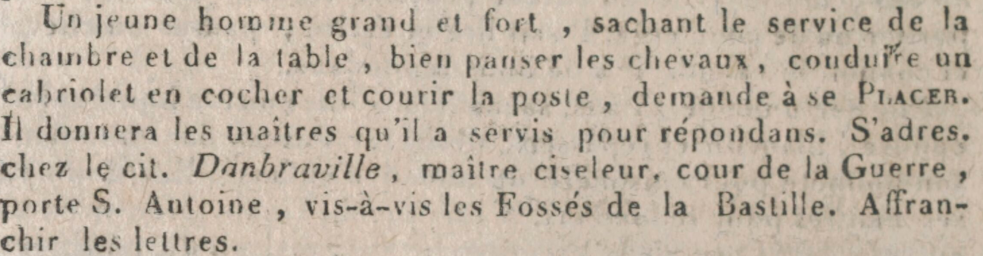
\includegraphics[width=12cm]{exemple_segmentation.png}
	\caption[Exemple d'annonce posant problème lors de la segmentation]{Exemple d'annonce posant problème lors de la segmentation: la première expression régulière coupe l'annonce en trois (après "PLACER." et après "S'adres."); la nouvelle expression régulière ne permet pas de pallier au problème de la première coupure, mais permet de contourner la seconde (\textit{Affiches de Paris}, 24 février 1804, p.8).}
\end{figure}

\begin{figure}[ht]
	\centering
	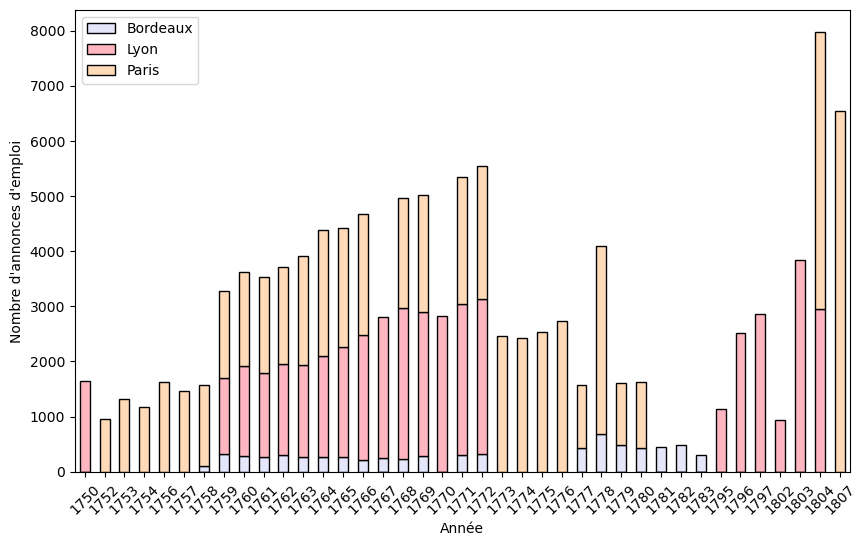
\includegraphics[width=12cm]{nb_annonces_tout_par_ville.png}
	\caption{Nombre d'annonces publiées par an selon la ville}
\end{figure}



\section{Des annonces aux annonces d'emploi: le processus de sélection}

Une fois les annonces isolées, il s'agissait ensuite de sélectionner parmi elles uniquement les annonces d'emploi. Pour ce faire, j'ai encore une fois privilégié l'usage d'une expression régulière. Après avoir lu plusieurs dizaines d'annonces, aussi bien dans les éditions parisiennes, bordelaises que lyonnaises des \textit{Affiches}, j'ai observé que la présence des expressions « se placer », « être placé » ou « une place » est le critère le plus déterminant dans la classification entre les annonces d’emploi et les autres annonces. D'où l'expression régulière suivante : \fbox{(une|être|se) place?é?r?"}. Après plusieurs tests, j'ai également observé que cette méthode incluait beaucoup d'annonces de voyages ou de ventes de voitures ("On offre une place dans une chaise de poste...", "On vend un cabriolet à une place..."); j'ai alors défini une expression spécifique pour en exclure une partie du corpus final.


\begin{figure}[ht]
	\centering
	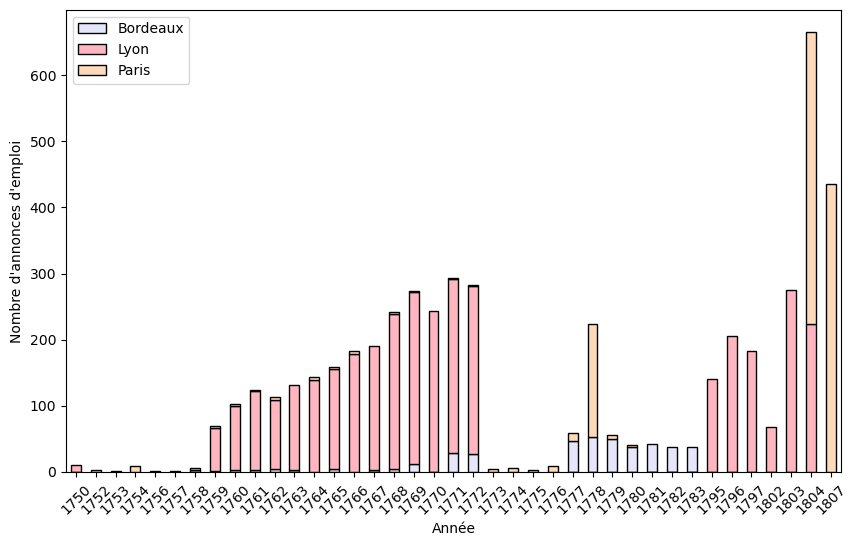
\includegraphics[width=12cm]{nb_annonces_emploi_par_ville.png}
	\caption{Nombre d'annonces d'emploi publiées par an selon la ville}
\end{figure}


\section{Des annonces d'emploi au  \textit{dataframe}: le choix du mode de stockage des données}

La méthode que j'ai décrit jusqu'ici a permis d'extraire 5064 annonces d'emploi à partir des journaux numérisés. Une dernière étape de la constitution du corpus consistait à choisir le meilleur format de stockage des annonces. Afin de préserver le maximum de métadonnées (date, ville de publication, ...), j'ai choisi de les stocker sous forme de \textit{dataframe pandas}, c'est-à-dire de tableau à deux dimensions. Le corpus initial prend donc la forme d'un tableau dont les colonnes sont: la ville de publication, l'année, le mois et le jour de publication, le texte de l'annonce. 
À partir de ce premier \textit{dataframe}, j'ai pu effectuer quelques traitements à l'aide de spacy et ajouter plusieurs colonnes: texte lemmatisé, texte sans mots vides, longueur. Ce examen initial des annonces a permis de produire de premiers résultats, limités mais qui donnent une vue d'ensemble du corpus. 

J'ai tout d'abord extrait les lemmes les plus fréquents du corpus, qui montrent bien l'uniformité des annonces entre elles: la présence de "adresser" dans plus de quatre annonces sur cinq, de "demande" et "désire" dans plus d'une sur trois, sont autant d'indices qui impliquent l'existence d'un script formel employé par le journal au moment du recueillement de la demande d'emploi. 

\begin{table}[ht]
	\parbox{.45\linewidth}{
		\centering
		\begin{tabular}{lc}
			\hline
			\multicolumn{1}{c}{\textbf{Lemme}} & \multicolumn{1}{c}{\textbf{Occurrences}} \\ \hline
			adresser                           & 4407                                      \\
			place                              & 3245                                      \\
			rue                                & 3167                                      \\
			placer                             & 2672                                      \\
			bon                                & 2510                                      \\
			maison                             & 1780                                      \\ 
			homme                              & 1780                                      \\ 
			demande                            & 1701                                      \\ 
			désirer                            & 1640                                      \\ 
			trouver                            & 1586                                      \\ \hline
		\end{tabular}
	}
	\hfill
	\parbox{.45\linewidth}{
		\centering
		\begin{tabular}{lc}
			\hline
			\multicolumn{1}{c}{\textbf{Lemme}} & \multicolumn{1}{c}{\textbf{Occurrences}} \\ \hline
			jeune                              & 1498                                      \\ 
			faire                              & 1485                                      \\ 
			donner                             & 1422                                      \\ 
			bien                               & 1307                                      \\ 
			écrire                             & 1277                                      \\ 
			ville                              & 1108                                      \\ 
			qualité                            & 989                                       \\ 
			degré                              & 914                                       \\ 
			entendre                           & 906                                       \\ 
			femme                              & 869                                       \\   \hline
		\end{tabular}
	}
	\caption{Vingt mots les plus fréquents du corpus lemmatisé et sans stopwords}
\end{table}


\begin{figure}[h]
	\centering
	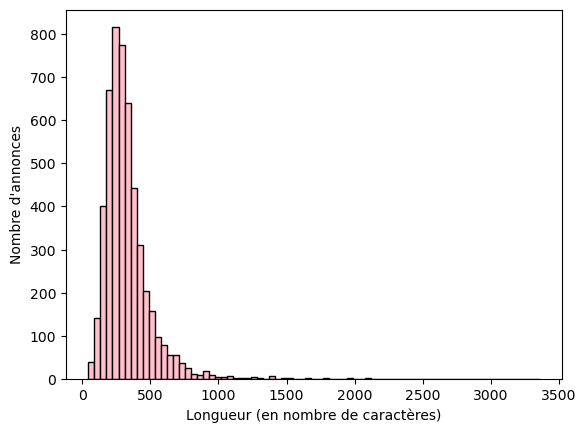
\includegraphics[width=12cm]{longueur.png}
	\caption{Répartition des annonces selon leur longueur}
\end{figure}

J'ai également pu à partir de ce premier dataframe m'intéresser à la longueur des annonces. Celle-ci est très homogène: plus de trois annonces sur quatre font entre 200 et 400 caractères, avec une médiane à 292 caractères. La norme formelle de l'annonce s'accompagne donc d'une norme de longueur, la petite annonce étant caractérisée par une brièveté qui garantit aussi la rentabilité du modèle des \textit{Affiches}.

Enfin, je souhaitais également m'intéresser lors des explorations préliminaires du corpus au phénomène de répétition et de republication des annonces, qui m'était apparu comme relativement important lors de mes lectures proches des journaux. Face à la gratuité de la publication, rien n'empêche de fait les domestiques en recherche d'emploi de proposer plusieurs fois leurs services dans plusieurs numéros différents, surtout si leur première demande s'est soldée par un échec. Néanmoins, la recherche automatique des annonces "doublons", grâce à la fonction "duplicated" de la librairie pandas appliquée aux annonces nettoyées, n'a pas portée ses fruits: seules 74 annonces sont extraites. Ces dernières sont pour la plupart republiées une seule fois; quelques annonces isolées sont répétées trois ou quatre fois, le plus souvent dans des numéros adjacents, ou dans le même mois. Des micro-variations typographiques, déjà présentes entre les annonces ou résultant de l'océrisation, expliquent probablement cette impossibilité d'extraire plus d'annonces répétées. Une autre solution, que je n'ai pas exploré ici, aurait pu être de s'intéresser à la répétition des adresses, seule partie de l'annonce qui est a priori garantie de ne pas être modifiée.